\chapter{Conclusions and Future Work}

\section{Usage Statistics}

This project was tested during the Deusto's ForoTech engineering week (figure~\ref{fig:forotech}).
During that testing that lasted for 8 days, hundreds of students saw the system. There was a live
demo in the forum itself, where students learned how to play the game and received their own user
and password to play from home. During those demonstrations, the experiment was used 72 times, with
a total of 16,119.5 seconds of use (about 4 hours and a half).

\begin{figure}[ht]
	\centering
	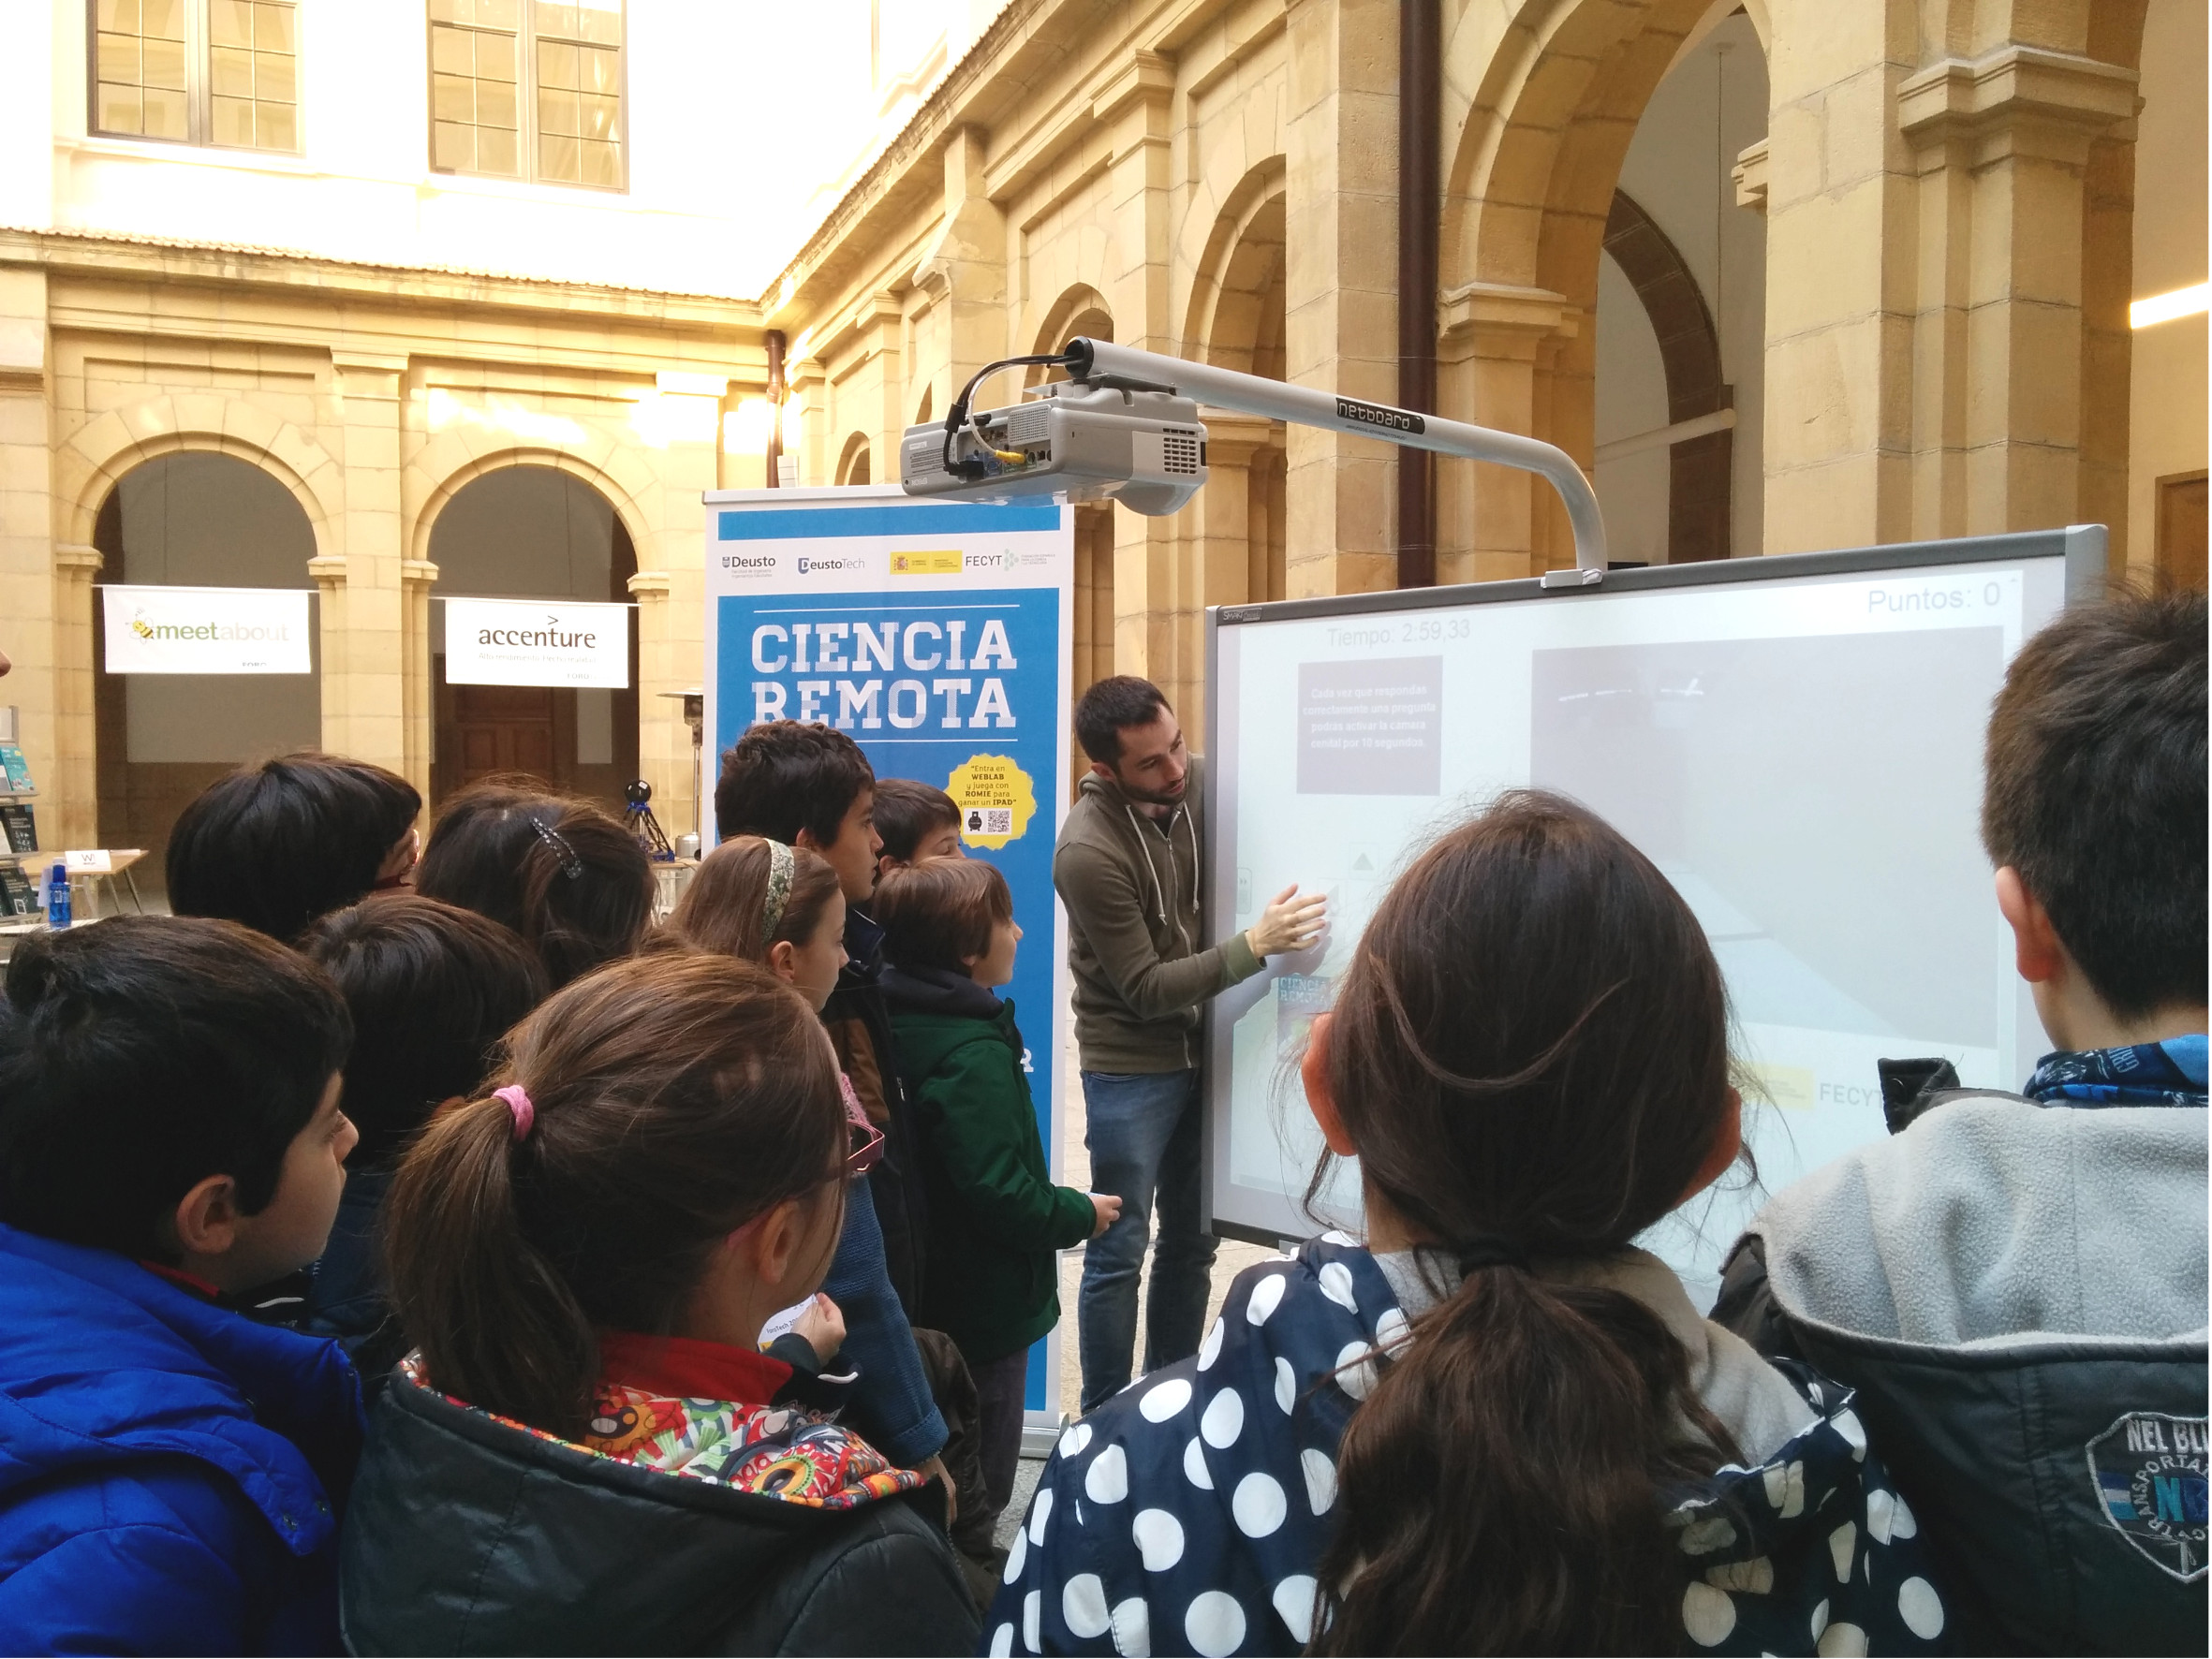
\includegraphics[height=0.3\textheight]{fig/forotech}
	\caption{Students looking at the ForoTech demonstration.}
	\label{fig:forotech}
\end{figure}

Moreover, 64 users logged in and played from home, with a total of 665 uses (more than 10 times per
user) with a total of 145,155.22 seconds of use (about 40 hours and 19 minutes), which is about
2,268 seconds per user or about 38 minutes.

The average game was of about 200 seconds (about 3 minutes and 20 seconds) and the day with most
uses was the Wednesday (the first day of use) in the afternoon, where the system had 164 uses. There
were no important issues with the robot, and most of them were hardware related, due to failing
pieces that were changed.

The final top ten ranking of the competition was the one in table~\ref{tab:ranking}. The first two
received an iPad (figure~\ref{fig:prizes}). There was a real competition where users were playing
until the last second of the competition, literally.

\begin{table}[ht]
	\centering
	\caption{Romie competition top ten ranking.}\label{tab:ranking}
	\begin{tabular}{ccc}
		\toprule
		\textbf{Name} & \emph{School} & \textbf{Points} \\
		\midrule
		Telmo		& Jesuitas					& 6,917,714	\\
		Hodei		& Jesuitas					& 6,915,484	\\
		Joshua		& El Regato					& 728,968	\\
		Martin		& Jesus María Bilbao		& 700,010	\\
		Adair		& Gurutzeta Eskola			& 589,400	\\
		Irune		& Jesuitas					& 578,420	\\
		Aitziber	& Jesuitas					& 464,070	\\
		Raul		& Fontal Somorrostro		& 456,865	\\
		Joseba		& Jesuitas					& 322,500	\\
		Antón		& Liceo Francés de Bilbao	& 221,520	\\
		\bottomrule
	\end{tabular}
\end{table}

\begin{figure}[ht]
	\centering
	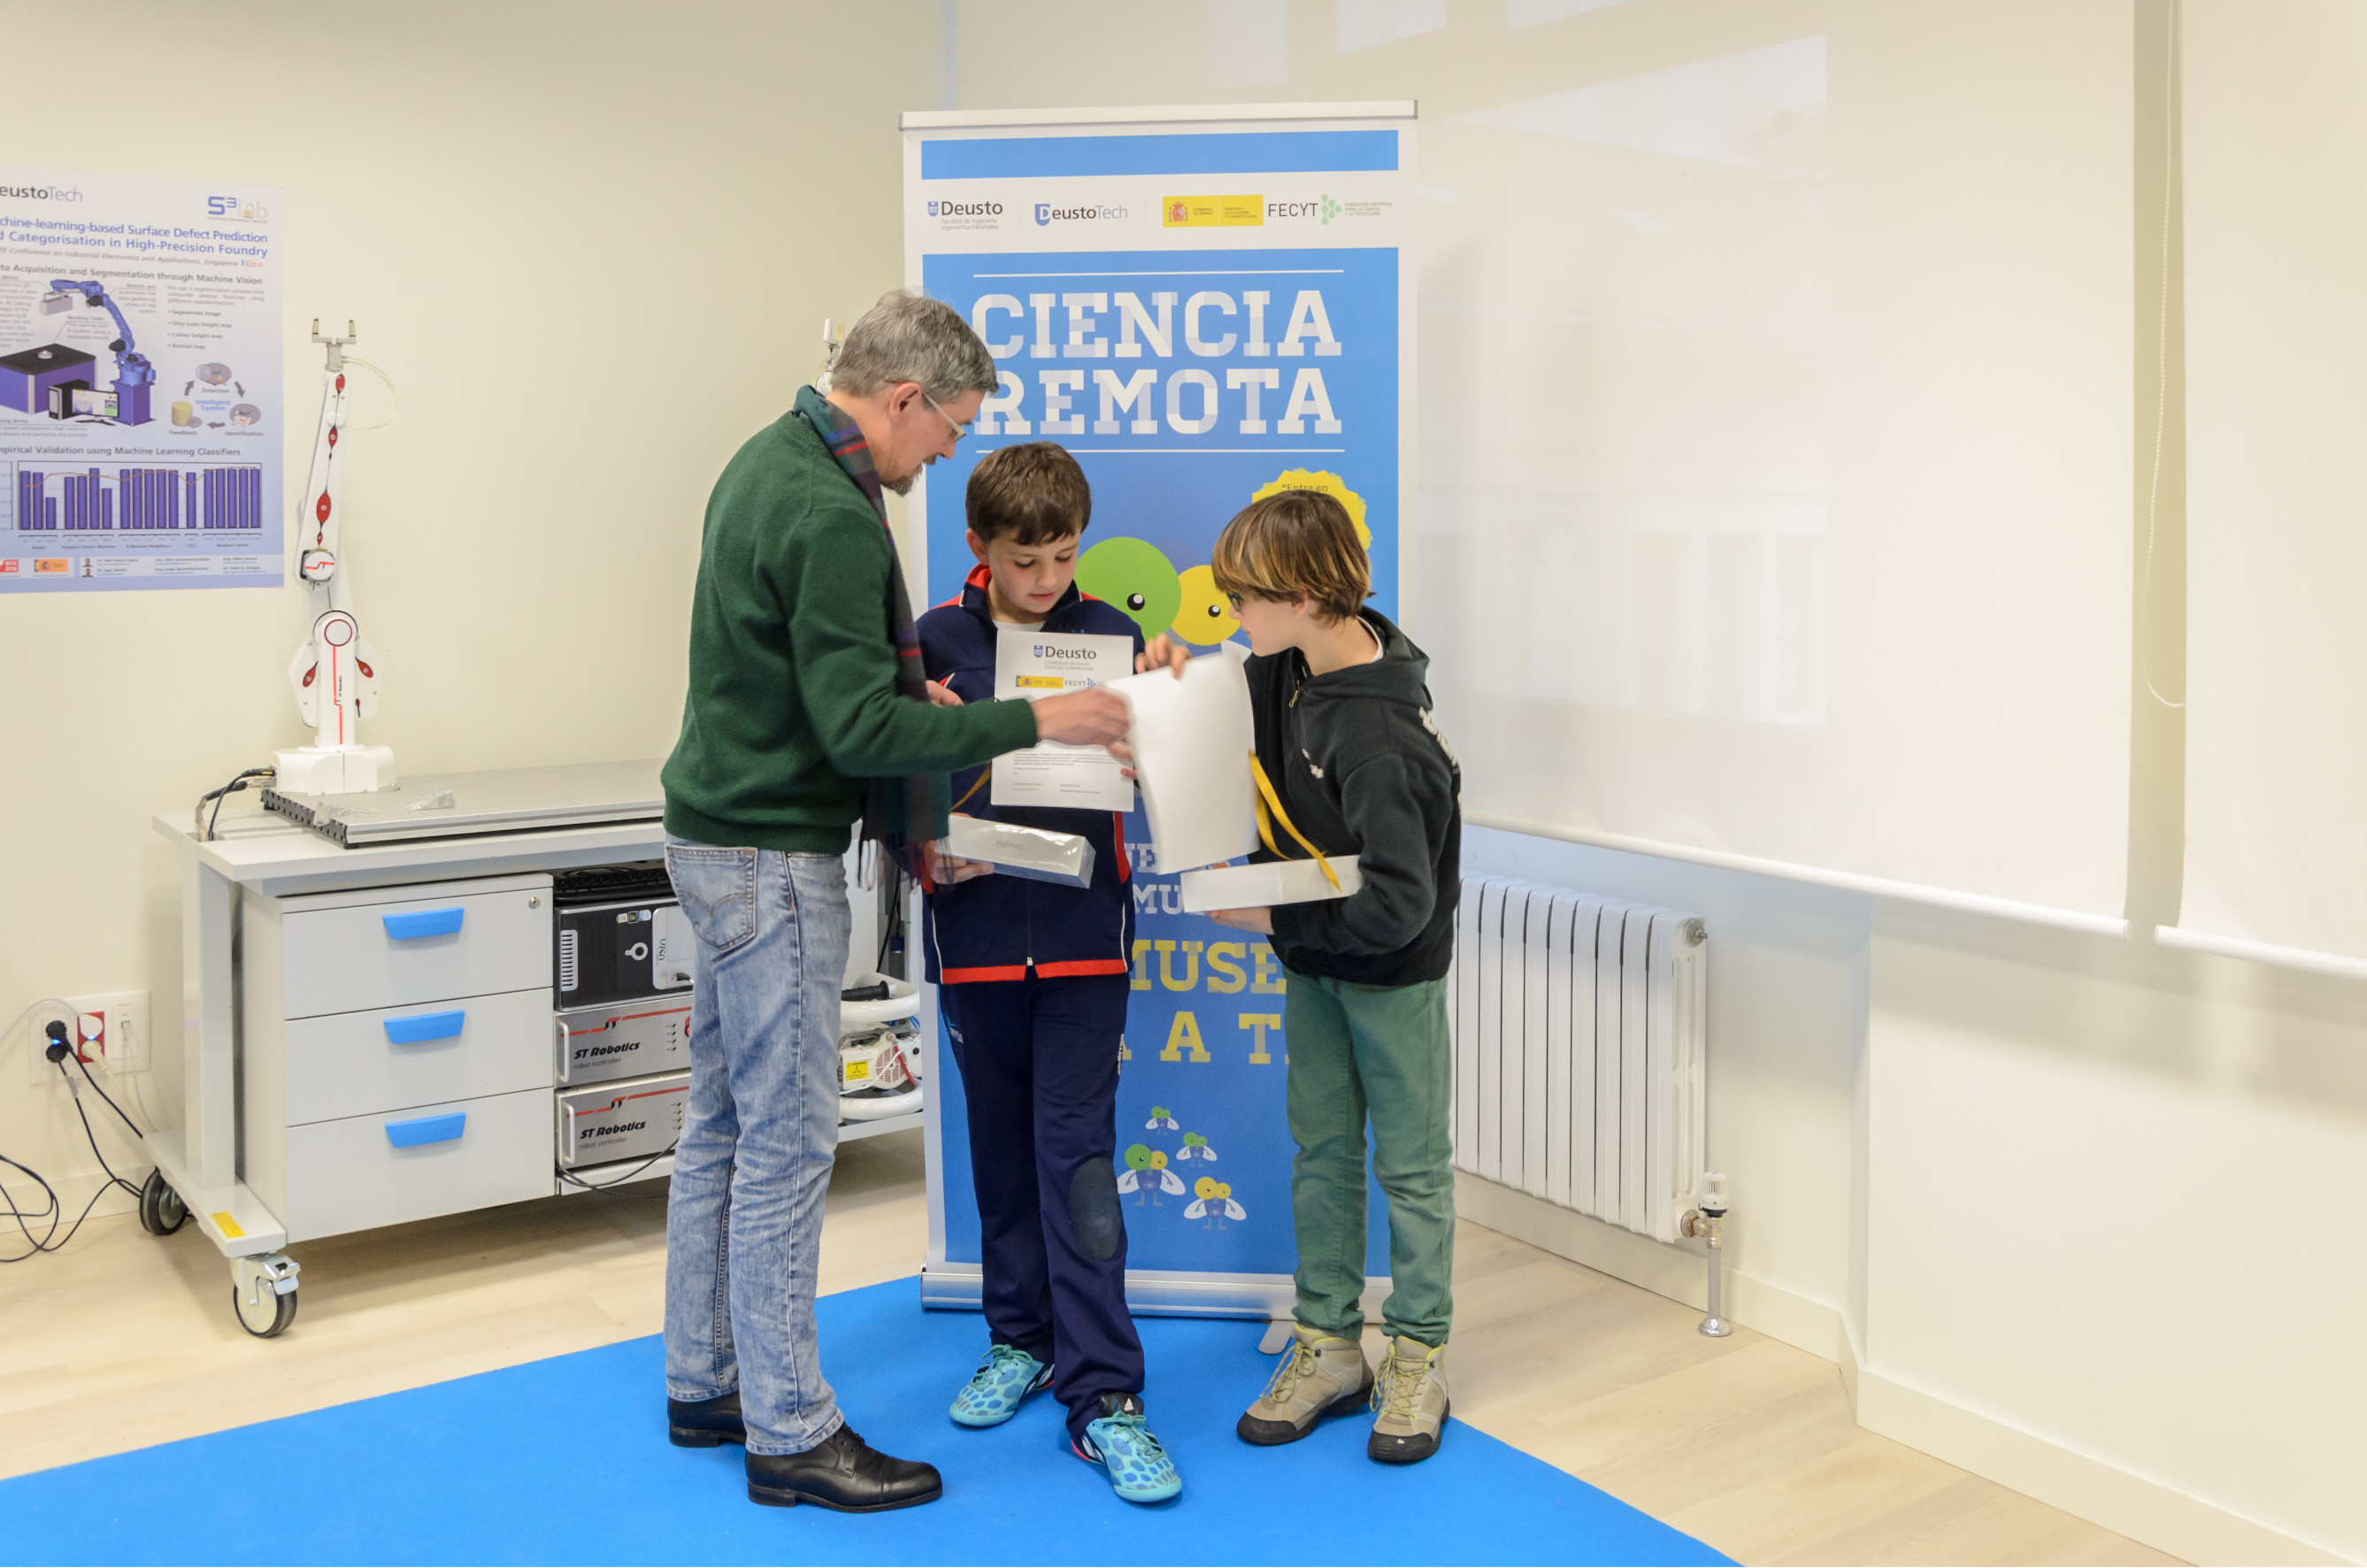
\includegraphics[height=0.3\textheight]{fig/prizes}
	\caption{Telmo and Hodei receiving the prize for wining the competition sponsored by \acrshort{fecyt}.}
	\label{fig:prizes}
\end{figure}

\section{Conclusions}

TODO: Conclusions

\section{Future Lines of Work}

The current work is a complete system with its game modes. In WebLab-Deusto is currently deployed in
production, so it can be considered finished. Nevertheless, there are many ways that could lead to
improve both the user experience and the results of this project. For instance, here are a few that
could be developed in future research:

\begin{itemize}

\item \textbf{Augmented reality}: The experiment could be equipped with augmented reality to give
more interactivity to the user. It could show any sort of 3D game information in the labyrinth. Some
scenarios have been suggested, such as a game where the user would have to recover things from the
labyrinth moving across all of it and use them to build other hardware. The possibilities are
unimaginable.

\item \textbf{Computer vision}: Computer vision could be added to both top and on-board cameras.
This way, the user and the software developed could have more information about the position of the
robot or even about information in the labyrinth.

It could help putting \acrshort{qr} or
\acrlong{qr} codes in the walls to show something to the user. Moreover, top camera's computer
vision could be used to locate the robot and try to challenge the user to move to a concrete place.

\item \textbf{New game modes}: The platform currently provides a trivial type game, to which a
psychological experiment can be added through configuration (is not enabled by default) and a visual
programming \acrshort{ide}, where the user can program the robot. Nevertheless, these are only
examples of the potential of this project.

The platform is prepared, thanks to its modular \acrshort{api}s to host more experiments and games
that could use it. It could be used for teaching, for experimenting with art (painting the walls or
asking the user to paint patterns with the robot movement) or for any other use the imagination can
lead us to.

\end{itemize}

In any case, the current platform is extensible enough to allow all kind of experiment development,
also allowing for remote deployments of more experiments like this one. In this case, we already
are planning to deploy the experiment in the Domus museum in A Coruña, Spain. This way, we can
demonstrate that the project has a big potential and that the future lines of work can lead it to
be used in many scopes.
